\documentclass{article} % For LaTeX2e
\usepackage{nips14submit_e,times}
\usepackage{amsmath}
\usepackage{amsthm}
\usepackage{amssymb}
\usepackage{mathtools}
\usepackage{hyperref}
\usepackage{url}
\usepackage{algorithm}
\usepackage[noend]{algpseudocode}
%\documentstyle[nips14submit_09,times,art10]{article} % For LaTeX 2.09

\usepackage{graphicx}
\usepackage{caption}
\usepackage{subcaption}

\def\eQb#1\eQe{\begin{eqnarray*}#1\end{eqnarray*}}
\def\eQnb#1\eQne{\begin{eqnarray}#1\end{eqnarray}}
\providecommand{\e}[1]{\ensuremath{\times 10^{#1}}}
\providecommand{\pb}[0]{\pagebreak}
\DeclarePairedDelimiter\ceil{\lceil}{\rceil}
\DeclarePairedDelimiter\floor{\lfloor}{\rfloor}

\newcommand{\E}{\mathrm{E}}
\newcommand{\Var}{\mathrm{Var}}
\newcommand{\Cov}{\mathrm{Cov}}

\def\Qb#1\Qe{\begin{question}#1\end{question}}
\def\Sb#1\Se{\begin{solution}#1\end{solution}}

\newenvironment{claim}[1]{\par\noindent\underline{Claim:}\space#1}{}
\newtheoremstyle{quest}{\topsep}{\topsep}{}{}{\bfseries}{}{ }{\thmname{#1}\thmnote{ #3}.}
\theoremstyle{quest}
\newtheorem*{definition}{Definition}
\newtheorem*{theorem}{Theorem}
\newtheorem*{lemma}{Lemma}
\newtheorem*{question}{Question}
\newtheorem*{preposition}{Preposition}
\newtheorem*{exercise}{Exercise}
\newtheorem*{challengeproblem}{Challenge Problem}
\newtheorem*{solution}{Solution}
\newtheorem*{remark}{Remark}
\usepackage{verbatimbox}
\usepackage{listings}
\usepackage{mathrsfs}
\title{Functional Analysis: \\
Problem Set I}


\author{
Youngduck Choi \\
CIMS \\
New York University\\
\texttt{yc1104@nyu.edu} \\
}


% The \author macro works with any number of authors. There are two commands
% used to separate the names and addresses of multiple authors: \And and \AND.
%
% Using \And between authors leaves it to \LaTeX{} to determine where to break
% the lines. Using \AND forces a linebreak at that point. So, if \LaTeX{}
% puts 3 of 4 authors names on the first line, and the last on the second
% line, try using \AND instead of \And before the third author name.

\newcommand{\fix}{\marginpar{FIX}}
\newcommand{\new}{\marginpar{NEW}}

\nipsfinalcopy % Uncomment for camera-ready version

\begin{document}


\maketitle

\begin{abstract}
This work contains solutions to the exercises of the problem set I.
\end{abstract}

\bigskip

\begin{question}[1]
\hfill
\begin{figure}[h!]
  \centering
    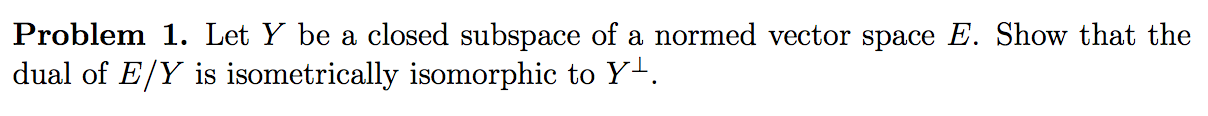
\includegraphics[width=0.7\textwidth]{funcA-h-e1-p1.png}
\end{figure}
\end{question}
\begin{solution} \hfill \\
First, define a map $\Phi:Y^{\perp} \to (E \setminus Y)^*$ naturally by
\eQb
f &\mapsto& ([x] \mapsto f(x))
\eQe 
where $[x] \in E\setminus Y$. The map is well-defined, because for any $[x] = [x']$,
\eQb
x' = x + y \>\> \text{for some} \>\> y \in Y \> \text{and} \>
f(x') = f(x) + f(y) = f(x).
\eQe
We now claim that $\Phi$ is a surjective isometry. By definition, for any $f \in
Y^{\perp}$,
\eQb
||\Phi(f)|| &=& \sup_{||[x]|| = 1} |<\Phi(f),[x]>| = \sup_{||[x]|| = 1} |<f,x>| \\
&=& \sup_{\inf_{y \in Y} ||x - y|| = 1} |<f,x>| 
\eQe 

\bigskip

For sake of completeness, we note that if both pre-image and image are Banach,
then a surjective isometry is a isometric isomorphism. This is a direct consequence
of open mapping theorem. First, isometry implies injectivity: for $T \in
\mathscr{L}(E,F)$ and $x,y \in E$, if $T(x) = T(y)$,
then $0 = ||T(x-y)|| = ||x-y||$, so $x = y$. Therefore, $T^{-1}$ is well-defined
as a map. Now, by open mapping theorem, we see that for any $O$ open in $E$,
$(T^{-1})^{-1}(O) = T(O)$ is open in $F$. Therefore, $T^{-1}$ is continuous as required.

\bigskip

It remains to be shown that $Y^{\perp}$ and $E \setminus Y$ are Banach. Suppose
$f \in E^*$ such that there exists $\{f_n\} \subset Y^{\perp}$ with $f_n \to f$. It
suffices to show that for any $y in Y$, we have $<f,y> = 0$. But this is true,
because norm convergence implies pointwise convergence and for all $n \geq 1$,
$<f_n,x> = 0$. Now, $E \setminus Y$ is Banach with respect to the quotient norm,
because  

\end{solution}

\newpage

\begin{question}[2]
\hfill
\begin{figure}[h!]
  \centering
    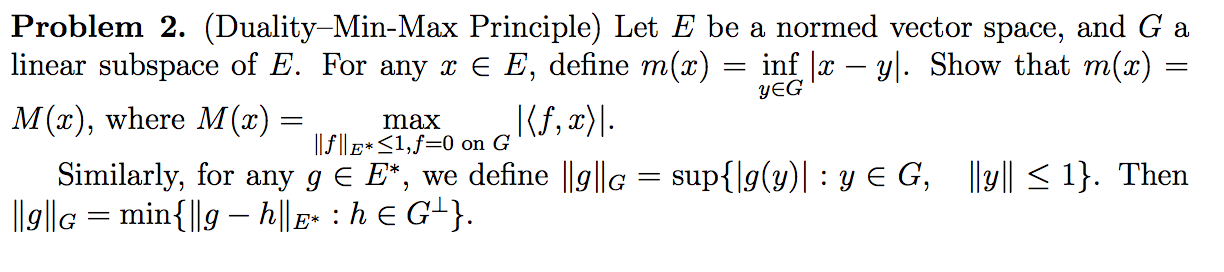
\includegraphics[width=0.7\textwidth]{funcA-h-e1-p2.png}
\end{figure}
\end{question}
\begin{solution} \hfill \\
If $x \in \bar{G}$, then $m(x) = 0$,
and $M(x) = 0$, because by continuity for any $f \in E^*$ such that $f = 0$
on $G$, it follows that $f = 0$ on $\overline{G}$.
Suppose $x \in  E \setminus \overline{G}$.  


\bigskip


\end{solution}

\newpage

\begin{question}[3]
\hfill
\begin{figure}[h!]
  \centering
    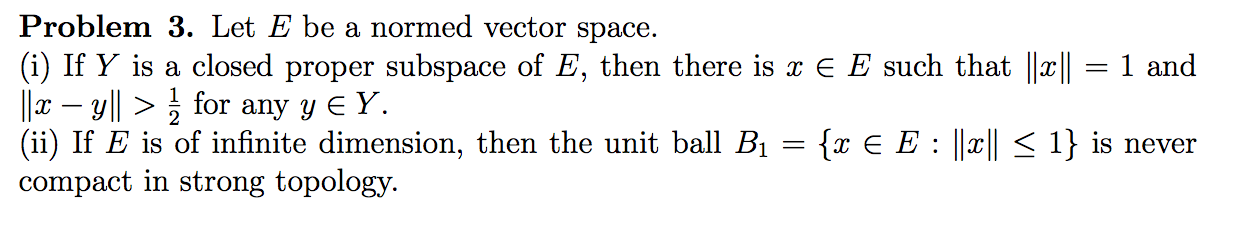
\includegraphics[width=0.7\textwidth]{funcA-h-e1-p3.png}
\end{figure}
\end{question}
\begin{solution} \hfill \\
\textbf{(i)} We prove the following generalization, known as the Riesz Lemma:
for each $\epsilon > 0$, there exists $x \in E$ such that $||x - y|| 
\geq 1 - \epsilon$, for any $y \in Y$. 

\smallskip

Let $0 < \epsilon < 1$. Let $x \in E\setminus Y$. As $Y$ is closed,
\eQb
d &:=& \text{dist}(x,Y) > 0.
\eQe
Choose $y^*$ in $Y$ such that 
\eQb
d \leq || x - y^* || \leq \dfrac{d}{1-\epsilon}. \>\>\> (1)
\eQe
Set $x^* = \dfrac{x-y^*}{||x-y^*||}$. Clearly, $||x^*|| = 1$, and,
for any $y \in Y$,
\eQb
||x^* - y|| &=& ||\dfrac{x-y^*}{||x-y^*||} - y|| = 
\dfrac{1}{||x-y^*||}||x- (y^* + y||x-y||^*)|| \\
&\geq&  \dfrac{d}{||x-y^*||} \leq 1-\epsilon, 
\eQe 
where the last inequality follows from $(1)$, and we are done. \hfill $\qed$ 

\bigskip

\textbf{(ii)} We proceed to construct a sequence $\{x_n\} \subset B_1$ 
such that there is no convergent subsequence, which shows that $B_1$ is not
compact in strong topology through sequential characterization of compactness
(strong topology is trivially metrizable). 

\smallskip
Choose any $x \in E$ such that $||x|| = 1$ and set $x_1 = x$. 
Then, for any $n$, using $(i)$, 
choose $x_n$ such that 
\eQb
||x_n|| = 1 \>\> \text{and}  \>\> ||x_n - y|| > \dfrac{1}{2}, 
\eQe
for any $y \in \text{span}(x_1,...,x_{n-1})$, where the validity comes from
the fact that any finite dimensional subspace is a proper, closed subspace
of an infinite dimensional space. Then, it is clear that $\{x_n\}$ has no
convergent subsequence, because for any $n \geq 1$, there exists $k, l \geq n$
with $k \neq l$, such that $||x_k - x_l|| > \dfrac{1}{2}$. Since being cauchy
is a necessary condition for being convergent, we are done. 
\hfill $\qed$ 

\end{solution}

\newpage

\begin{question}[4]
\hfill
\begin{figure}[h!]
  \centering
    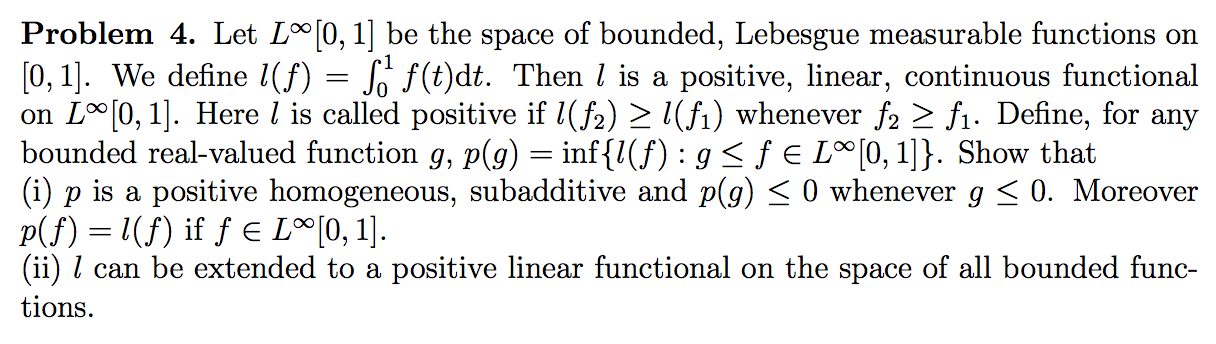
\includegraphics[width=0.7\textwidth]{funcA-h-e1-p4.png}
\end{figure}
\end{question}
\begin{solution} \hfill \\
\textbf{(i)} 
Let $g$ be a bounded real-valued function and $\lambda > 0$. Then, by
linearity of Lebesgue integration,
\eQb
p(\lambda g) &=& \inf\{ l(h): \lambda g \leq h \in L^{\infty} \} \\
\lambda p(g) &=& \inf\{ l(\lambda h): g \leq h \in L^{\infty} \}.
\eQe
We claim that
\eQb
A := \{ l(h) : \lambda g \leq h \in L^{\infty} \} &=& 
\{ l(\lambda h): g \leq h \in L^{\infty} \} =: B
\eQe
If $\lambda g \leq h \in L^{\infty}$, 
then $ g \leq \dfrac{h}{\lambda} \in L^{\infty}$,
so $l(\lambda \dfrac{h}{\lambda}) = l(\lambda) \in B$. Conversely, if 
$ g \leq h \in L^{\infty}$ then, $\lambda g \leq \lambda h \in L^{\infty}$, 
so $l(\lambda h) \in A$. Hence, $p(\lambda g) = \lambda p(g)$. 

\smallskip

We now show that $p$ is sub-additive. Let $f,g$ be bounded real functions.
Then, for any $h_1, h_2 \in L^{\infty}$ such that $f \leq h_1$ and $g \leq h_2$,
\eQb
f+g &\leq& h_1 + h_2 \in L^{\infty},
\eQe
so, again by linearity of integration, 
\eQb
p(f+g) &\leq& l(h_1 + h_2) = l(h_1) + l(h_2). 
\eQe
Taking infs for $h_1$, then $h_2$, gives
\eQb
p(f+g) &\leq& p(f) + p(g), 
\eQe
as required.

\smallskip
 
For any $f,g$ bounded real-valued functions, 
\eQb
p(f+g) &=& \inf\{ l(f+g) : f+g \leq h , h \in L^{\infty}[0,1]\} \\ 
&=& \inf\{ l(f) + l(g) : f+g \leq h , h \in L^{\infty}[0,1]\}. 
\eQe
Suppose $g \leq 0$. Then, as $0 \in L^{\infty}[0,1]$ and $l(0) = 0$, by definition,
$p(g) \leq 0$. 

\smallskip

We show that $p(f) = l(f)$ if $f \in L^{\infty}[0,1]$. 
For all $h \in L^{\infty}[0,1]$ such that $f \leq h$, then, by monotonicity
of Lebesgue integration, $l(f) \leq l(h)$. Since $f \leq f$ trivially, it follows
that $p(f) = l(f)$. \hfill $\qed$

\bigskip

\textbf{(ii)}
Now, as $l = p$ on $L^{\infty}[0,1]$, by Hahn-Banach, $l$ can be extended to
the entire space of bounded real-valued functions. This shows that 
we can make sense of integration for any bounded functions in a weaker sense,
sacrificing some nice properties, such as countable additivity and so on(probably
if such properties hold, then it will contradict existence of non-measurable sets
by considering appropriate indicators). 
\hfill $\qed$ 
\end{solution}

\newpage

\begin{question}[5]
\hfill
\begin{figure}[h!]
  \centering
    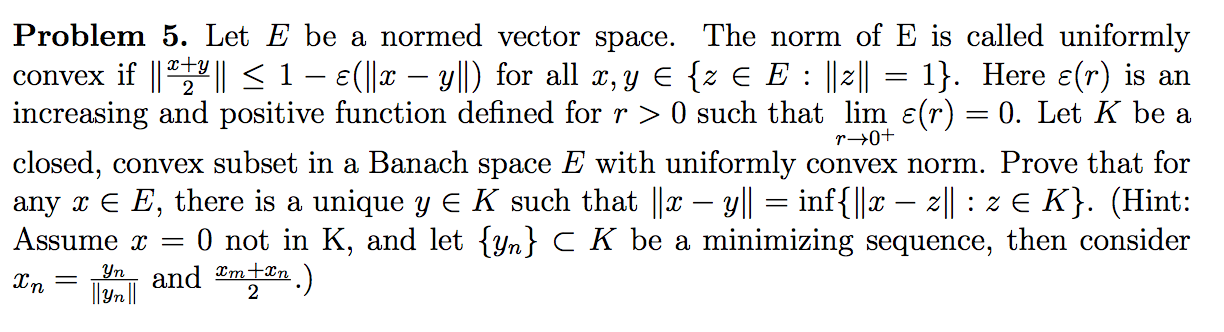
\includegraphics[width=0.7\textwidth]{funcA-h-e1-p5.png}
\end{figure}
\end{question}
\begin{solution} \hfill \\
Without loss of generality, assume $x = 0$ and $x \not \in K$. Let $\{y_n\}$
be the minimizing sequence. As $E$ is Banach, and $K$ is closed, it suffices to 
show that $\{y_n\}$ is cauchy. We claim that, it suffices to show, 
\eQb
||\dfrac{x_n + x_m}{2}|| \to 1 \>\>\> \text{as} \>\>\> n,m \to \infty \>\> (*)
\eQe 
By uniform convexity assumption, the above implies that $\{x_n\}$ is cauchy.
Now, it follows that that $\{y_n\}$ is cauchy.

\bigskip

Now, we prove $(*)$. 
by convexity of $K$, for any $n,m \geq 1$,
\eQb
d \leq ||\dfrac{y_n + y_m}{2}|| \leq ||\dfrac{y_n}{2}|| + ||\dfrac{y_m}{2}|| 
\eQe
so
\eQb
||\dfrac{y_n + y_m}{2}|| \to d \>\>\> &\text{as}& \>\> n,m \to \infty.
\eQe
Then,
\eQb
\lim_{n,m \to \infty} ||\dfrac{x_n + x_m}{2}|| &=& 
||\lim_{n \to \infty}\dfrac{y_n}{2||y_n||} + \lim_{n \to \infty}\dfrac{y_m}{2||y_m||}||
= \dfrac{1}{d} ||\lim_{n\to \infty} \dfrac{y_n}{2} + \lim_{m \to \infty}
\dfrac{y_m}{2}|| \\ 
&=& \dfrac{1}{d} \lim_{n,m \to \infty} || \dfrac{y_n + y_m}{2} || = 1 \\ 
\eQe
and we are done. \hfill $\qed$

\end{solution}

\newpage

\begin{question}[6]
\hfill
\begin{figure}[h!]
  \centering
    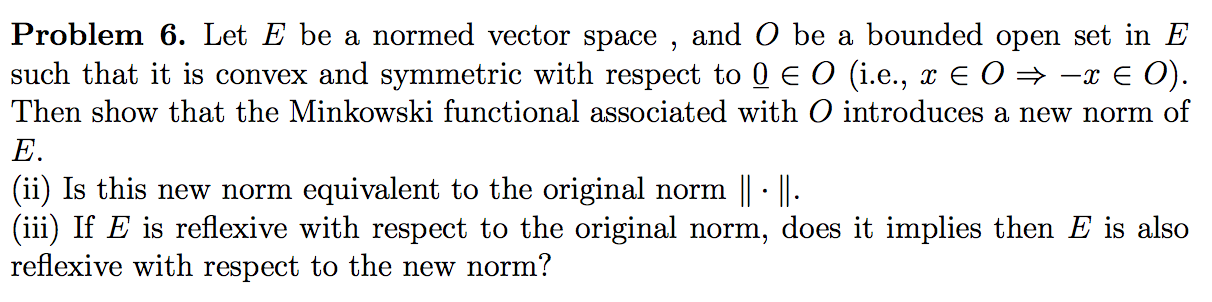
\includegraphics[width=0.7\textwidth]{funcA-h-e1-p6.png}
\end{figure}
\end{question}
\begin{solution} \hfill \\
By ordinary properties of Minkowski functionals, it suffices to show that
for any $x \in E$ and $\lambda \in \mathbb{R}$,
\eQb
p(\lambda x) = |\lambda| p(x) \>\> &\text{and}& \>\>
p(x) = 0 \implies x = 0.
\eQe
We first prove the absolute homogeneity of $p$.
Now, if $\lambda \geq 0$,
then $p(\lambda x) = \lambda p(x)$ by positive homogeneity of Minkowski functionals.
Now, if $\lambda \geq 0$, then, by symmetry, and positive homogeneity again,
we obtain
\eQb
p(\lambda x) = p(-\lambda x) = -\lambda p(x), 
\eQe
which completes the proof of absolute homogeneity. 

\bigskip

Now, observe that, for any $0 <\alpha < \beta$, and $x \in E$, 
\eQb
\alpha^{-1}x \in C &\implies \beta^{-1}x \in C,
\eQe
because by convexity
\eQb
(1- \dfrac{\beta^{-1}}{\alpha^{-1}})0 + \dfrac{\beta^{-1}}{\alpha^{-1}}\alpha^{-1}x
= \beta^{-1}x \in C.
\eQe
Let $x \in E$ such that $p(x) = 0$, Then, by the above discussion,
it follows that
\eQb
\alpha^{-1}x &\in& C \>\>\> (*),
\eQe
for any $\alpha \in (0,\infty)$. Suppose $x \neq 0$, and let $r > 0$ 
large enough that $C \subset B(0,r)$. Then, it follows that, from $(*)$,
$\dfrac{r}{||x||}x \in C$, which contradicts the fact that $C \subset B(0,r)$.
Therefore, $x = 0$ and we are done. \hfill $\qed$

\bigskip

\textbf{(i)} The norm is equivalent 

\textbf{(ii)} Reflexive implies that the space is Banach (so there is no confusion
with definition). 

We prove the following claim: Let $E$ be Banach space that is reflexive. For
any normed linear space, defined by an equivalent norm on $E$, is reflexive.

\bigskip
Consider an equivalent norm. Since the norm is equivalent with the original norm,
the induced topology is equal to the original topology, 
hence the dual and induced weak topology coincide as well. We know that
Banach space is reflexive iff the closed unit ball is weakly compact. Now,
it suffices to show that, for any topology, compactness of the closed unit ball
$B_1$ implies, for any $c > 0$, $B_c$ is compact. Suppose $\{U_{\lambda}\}$ 
is a finite cover of $B_1$. Define $\{\tilde{U}_{\lambda}\}$ by 

 

\end{solution}

\newpage

\begin{question}[7]
\hfill
\begin{figure}[h!]
  \centering
    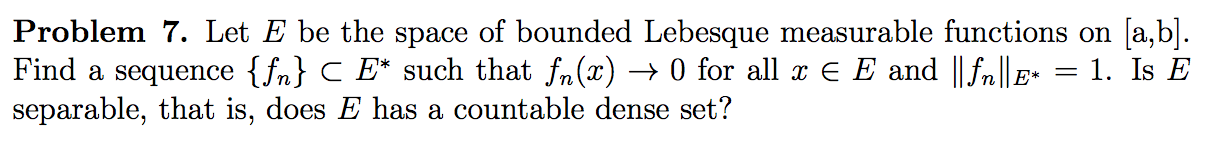
\includegraphics[width=0.7\textwidth]{funcA-h-e1-p7.png}
\end{figure}
\end{question}
\begin{solution} \hfill \\
Consider $\{f_n\}$ defined by
\eQb
g &\mapsto& \int_{\mathbb{T}} g(t)
e^{-2\pi i nt} dt = \hat{g}(n) \>\>\> (g \in L^{\infty}(\mathbb{T})) 
\eQe
for each $n \geq 1$.
As $L^{\infty}(\mathbb{T}) \subset L^{1}(\mathbb{T})$, 
by Riemann-Lebesgue lemma, for any $g \in L^{\infty}(\mathbb{T})$,
\eQb
f_n(g) = \hat{g}(n) \to 0. 
\eQe
For any $n \geq 1$, $g \in L^{\infty}(\mathbb{T})$ with $||g|| = 1$, 
\eQb
|\hat{g}(n)| &\leq& \int_{\mathbb{T}} |g| \leq ||g||_{\infty} = 1,
\eQe
Now, for any $n \geq 1$, take $g = e^{2\pi int}$ to see
\eQb
|\hat{g}(n)| &=& |\int_{\mathbb{T}} 1dt| = 1,  
\eQe 
so, combined with the above estimate, we have
\eQb
||f_n|| = 1,
\eQe
as required.

\bigskip

It is a well-known fact that $L^{\infty}$ is not separable, given 
that the ambient space is not finite. Instead of appealing to this general result,
we provide a construction of uncountable family of functions in $L^{\infty}[a,b]$
with $a <b$ 
such that the distance is at least 1 apart to contradict the separability assumption.
Take $[a,b]$ such that $a < b$. Fix $x_0 \in (a,b)$ and consider $
\mathscr{A} = \{1_{B(x_0,r)} \}$
where $0 < r \leq \min(x_0-a,b-x_0)$. Then, the family is uncountable, but for 
any $f,g \in \mathscr{A}$, 
\eQb
||f - g||_{\infty} &=& 1.
\eQe
Now, suppose the space is separable, hence there exists a countable dense subset
$C$. Now, observe that
\eQb
\bigcup_{x \in \mathscr{A}} B(x,\dfrac{1}{2}) \cap C \subset C,
\eQe 
but the left hand side is uncountable, because its an uncountable 
disjoint union of countable sets. Therefore, $L^{\infty}[a,b]$ is not separable. \hfill
$\qed$

 
\end{solution} 


\end{document}
